El salario ($S$), expresado en una unidad monetaria (como dinero en dolares \$, yuanes o euros), tiene un comportamiento lineal con respecto al tiempo ($t$), expresado en una unidad de tiempo (como horas $h$, meses o años). Esta relación, salario por hora ($r$), se expresa en unidades monetarias entre unidades de tiempo ($\$/h$). La expresión matemática es la siguiente:

\[
  r = \dfrac{S}{t} = \dfrac{\$}{h}
\]

El salario en función del tiempo se puede expresar de la siguiente forma:

\begin{listequbox}
  {S(t) = rt + S_0}{equsalariolin}{Salario en función del tiempo}
\end{listequbox}

En este caso el salario es constante en el tiempo.

\textbf{Elementos:}

\begin{itemize}
  \item \textbf{S(t)}: salario acumulado en el tiempo $t$.
  \item \textbf{$S_0$}: salario inicial o base, si lo hay.
  \item \textbf{r}: tasa de pago por unidad de tiempo.
  \item \textbf{t}: tiempo trabajado, expresado en la misma unidad que $r$.
\end{itemize}

Suponiendo un $r$ de 20, se obtiene la siguiente función:

\[
  S(t) = 20t
\]

Tabla de valores:

\begin{center}
\begin{tabular}{|c|c|c|c|c|c|c|c|c|}
  \hline
  S(\$) & 20 & 40 & 60 & 80 & 100 & 120 & 140 & 160 \\
  \hline
  t(h) & 1 & 2 & 3 & 4 & 5 & 6 & 7 & 8 \\
  \hline
\end{tabular}
\end{center}

Gráfica:

\begin{grafica}
\center
\begin{tikzpicture}
  \begin{axis}[
    xlabel=\text{Tiempo trabjado}\ $t(h)$,
    ylabel=\text{Salario}\ $S(\$)$,
    xmin=0,xmax=9,
    ymin=0,ymax=170,
    legend style={at={(0.5,0.8)}},
    axis lines=middle
    ]
  \addplot[color=blue,domain=0:8,thick]{x*20}
  node[right,pos=0.5,black,thick]{$r\left(\dfrac{\$}{h}\right)$};
  \addlegendentry{$S(t) = rt + S_0$}
\end{axis}
\end{tikzpicture}
\caption{Salario en función del tiempo}
\end{grafica}
